\chapter{Desenvolvimento}
\label{cap:desenvolvimento}

Este capítulo apresenta o desenvolvimento do estudo de caso com Microsserviços e \acrshort{ddd}. Ele descreve as etapas para construção do sistema a partir de requisitos funcionais e não-funcionais.

\section{Ciclo de Vida do Desenvolvimento de Software}
\citeonline{barbaraLiskov} descreve 6 etapas no ciclo de vida de um software: Análise de requisitos, \english{Design}, Implementação e Teste, Teste de aceitação, Produção e Manutenção. A Figura \ref{fig:ciclo-vida} ilustra essas etapas. 

\begin{figure}[H]
    \centering
    \caption{Ciclo de Vida do Desenvolvimento de Software}
    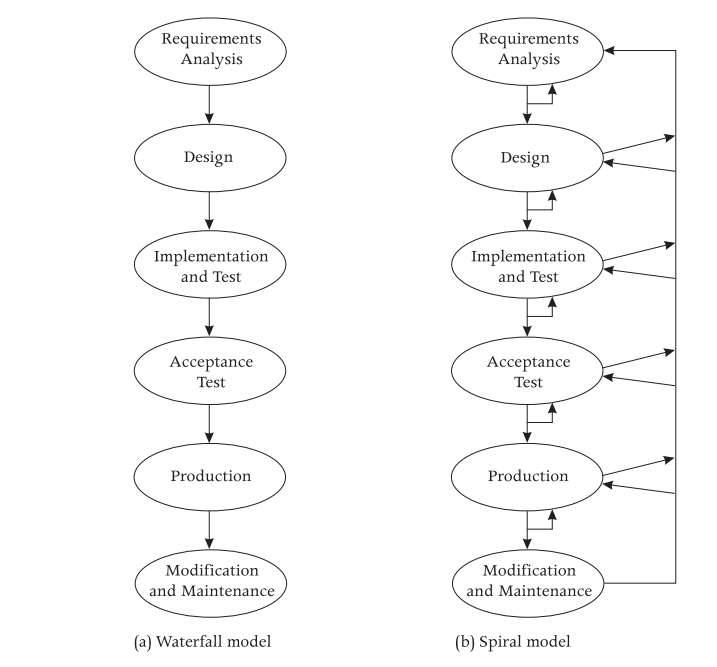
\includegraphics[width=0.8\textwidth]{media/software-life-cycle.png}
    \fonte{\citeonline{barbaraLiskov}}
    \label{fig:ciclo-vida}
\end{figure}

Para este trabalho, os requistos foram definidos no \autoref{cap:metodologia}. Da mesma forma, a fase de manutenção não será abordada, pois o foco é a construção do sistema.

\section{Design}
Esta seção utiliza como entrada os requisitos funcionais e não-funcionais definidos no \autoref{cap:metodologia} para descrever o design do sistema utilizando \acrfull{ams} e \acrfull{ddd}.

Inicialmente, é importante definir as abstrações chaves do sistema, bem como seus relacionamentos. A \autoref{fig:modelo_conceitual} ilustra as abstrações do sistema.

\begin{figure}[H]
    \centering
    \caption{Modelo conceitual do sistema}
    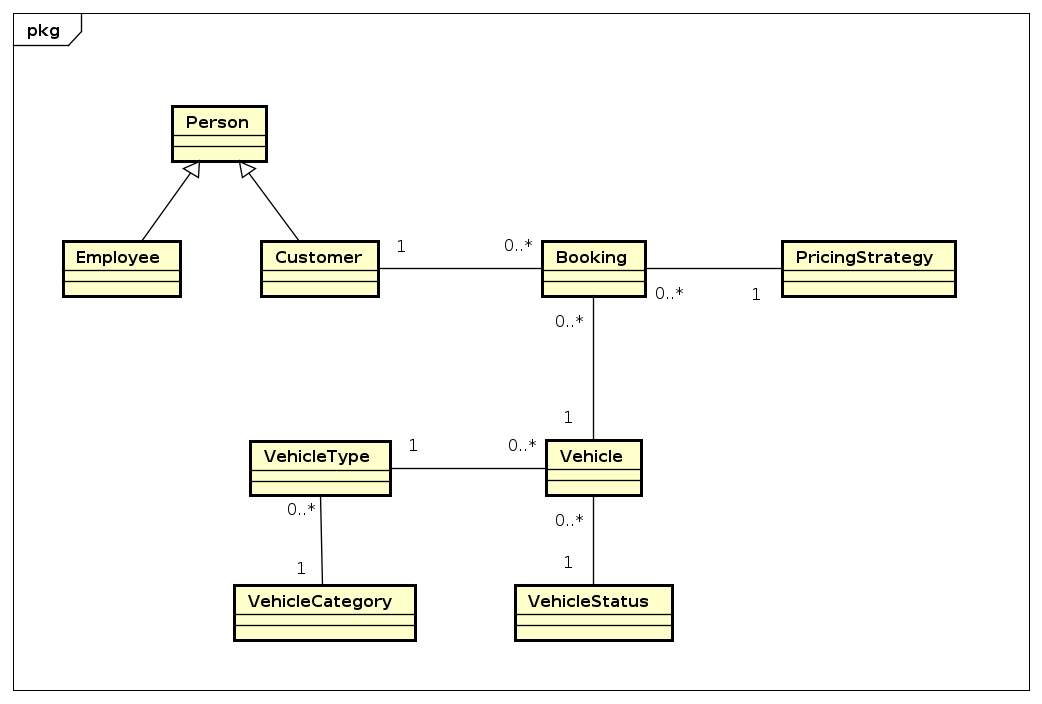
\includegraphics[width=0.8\textwidth]{media/modelo_conceitual.png}
    \fonte{o autor}
    \label{fig:modelo_conceitual}
\end{figure}
